\begin{figure}[H]
\centering
\includegraphics[page=6,width=0.33\textwidth]{\FCNCFigures/tthML/showFake/fakelep/fakeFactor/NOMINAL/reg2lSS1tau1bnj_os/lep_pt_1.pdf}
\put(-80, 80){\textbf{(a1)}}
\put(-100, 70){\tiny{$2lSS1tau1bnj$}}
\includegraphics[page=6,width=0.33\textwidth]{\FCNCFigures/tthML/showFake/fakelep/fakeFactor/NOMINAL/reg2lSS1tau1bnj_os_antiiso/lep_pt_1.pdf}
\put(-80, 80){\textbf{(b1)}}
\put(-100, 70){\tiny{$2lSS1tau1bnj~anti\-iso~sublead$}}
\includegraphics[page=6,width=0.33\textwidth]{\FCNCFigures/tthML/showFake/fakelep/fakeFactor/NOMINAL/reg2lSS1tau1bnj_os_antiisolead/lep_pt_1.pdf}
\put(-80, 80){\textbf{(c1)}}
\put(-100, 70){\tiny{$2lSS1tau1bnj~anti\-iso~lead$}}

\includegraphics[page=6,width=0.33\textwidth]{\FCNCFigures/tthML/showFake/fakelep/fakeFactor/NOMINAL/reg2lSS1taunj_os/lep_pt_1.pdf}
\put(-80, 80){\textbf{(a2)}}
\put(-100, 70){\tiny{$2lSS1taunj$}}
\includegraphics[page=6,width=0.33\textwidth]{\FCNCFigures/tthML/showFake/fakelep/fakeFactor/NOMINAL/reg2lSS1taunj_os_antiiso/lep_pt_1.pdf}
\put(-80, 80){\textbf{(b2)}}
\put(-100, 70){\tiny{$2lSS1taunj~anti\-iso~sublead$}}
\includegraphics[page=6,width=0.33\textwidth]{\FCNCFigures/tthML/showFake/fakelep/fakeFactor/NOMINAL/reg2lSS1taunj_os_antiisolead/lep_pt_1.pdf}
\put(-80, 80){\textbf{(c2)}}
\put(-100, 70){\tiny{$2lSS1taunj~anti\-iso~lead$}}\\

\caption{The distributions of lepton $p_{T}$ in the regions used for the FF.~~~~~~~~~~~}
\label{fig:fake_factors_sub}
\end{figure}